\documentclass[12pt,a4paper]{article}
\usepackage[utf8]{vietnam}
\usepackage{amsmath,amssymb}
\usepackage{geometry}
\geometry{top=1.5cm,bottom=1.2cm,left=1.4cm,right=1.4cm,headheight=28pt,headsep=12pt,footskip=18pt}
\usepackage{tikz}
\usepackage{xcolor}
\usepackage{enumerate}
\usepackage{graphicx}
\usepackage[version=4]{mhchem}
\usepackage{fancyhdr}
\usepackage{ex_test}

\renewcommand{\baselinestretch}{0.96}
\setlength{\parskip}{0pt}

\definecolor{hfRed}{RGB}{211,47,47}
\definecolor{hfGreen}{RGB}{139,195,144}

\pagestyle{fancy}
\fancyhf{}
\fancyhead[L]{\small\itshape\color{hfRed} Tài liệu lưu hành nội bộ}
\fancyhead[R]{\small\itshape\color{hfRed} Thầy \textbf{TRẦN VĂN THẠNH} - 0777.470.803}
\renewcommand{\headrulewidth}{0.8pt}
\renewcommand{\headrule}{\hbox to\headwidth{\color{hfGreen}\leaders\hrule height \headrulewidth\hfill}}

\fancyfoot[L]{\small\itshape\color{hfRed} CS1: 6/15 Nguyễn Hoàng, P. Kim Long, TP Huế \quad|\quad CS2: 24 Đặng Thái Thân, TP Huế}
\fancyfoot[R]{\small\bfseries\color{hfRed} Trang \thepage}
\renewcommand{\footrulewidth}{0.8pt}
\renewcommand{\footrule}{\hbox to\headwidth{\color{hfGreen}\leaders\hrule height \footrulewidth\hfill}}

\fancypagestyle{firstpage}{
  \fancyhf{}
  \renewcommand{\headrulewidth}{0pt}
  \fancyfoot[L]{\small\itshape\color{hfRed} CS1: 6/15 Nguyễn Hoàng, P. Kim Long, TP Huế \quad|\quad CS2: 24 Đặng Thái Thân, TP Huế}
  \fancyfoot[R]{\small\bfseries\color{hfRed} Trang \thepage}
  \renewcommand{\footrulewidth}{0.8pt}
  \renewcommand{\footrule}{\hbox to\headwidth{\color{hfGreen}\leaders\hrule height \footrulewidth\hfill}}
}

\begin{document}
\thispagestyle{firstpage}

\noindent
\begin{minipage}[t]{0.44\textwidth}
	\centering\fontsize{10pt}{12pt}\selectfont
	\textbf{SỞ GIÁO DỤC VÀ ĐÀO TẠO THỪA THIÊN HUẾ}\\
	\textbf{ĐỀ CHÍNH THỨC}\\
	\textit{(Đề thi có 04 trang)}
\end{minipage}\hfill
\begin{minipage}[t]{0.54\textwidth}
	\centering\fontsize{10.5pt}{13pt}\selectfont
	\textbf{ĐỀ KIỂM TRA ĐỊNH KỲ CHƯƠNG 3 (ĐẠI CƯƠNG HÓA HỮU CƠ)}\\
	\textbf{MÔN: HOÁ HỌC - LỚP 11}\\
	\textit{Thời gian làm bài: 45 phút, không kể thời gian phát đề}
	
	\smallskip
	\fbox{\textbf{MÃ ĐỀ: 108}}
\end{minipage}

\smallskip
\noindent\hrulefill
\smallskip

\noindent\textbf{Họ, tên thí sinh:} \dotfill\ \textbf{Lớp:} \dotfill\ \textbf{Số báo danh:} \dotfill

\smallskip
\noindent\textit{(Cho biết nguyên tử khối: H = 1; C = 12; N = 14; O = 16; F = 19; Na = 23; Mg = 24; Al = 27; P = 31; S = 32; Cl = 35,5; K = 39; Ca = 40; Fe = 56; Cu = 64; Br = 80; Ag = 108).}
\smallskip

\noindent\textbf{\large PHẦN I. Câu trắc nghiệm nhiều phương án lựa chọn.}
\textit{Thí sinh trả lời từ câu 1 đến câu 18. Mỗi câu hỏi thí sinh chỉ chọn một phương án.}
\vspace{0.2cm}

\Opensolutionfile{ans}[ans-hoa11-de08hs]

\begin{ex}
\textbf{[KNTT - SBT]} Xét phản ứng quang hợp: $\ce{6CO2 + 6H2O -> C6H12O6 + 6O2}$. Chất nào trong phản ứng này thuộc loại hợp chất hữu cơ?
\choice
{$\ce{CO2}$}
{$\ce{H2O}$}
{\True $\ce{C6H12O6}$}
{$\ce{O2}$}

\end{ex}

\begin{ex}
\textbf{[KNTT - SBT]} Hydrocarbon là loại hợp chất hữu cơ mà thành phần phân tử có các nguyên tố nào sau đây?
\choice
{\True C và H}
{C, H và O}
{C, H và N}
{C, H, O và N}

\end{ex}

\begin{ex}
\textbf{(SBT - CTST)} Phương pháp chưng cất dùng để tách các chất
\choice
{\True có nhiệt độ sôi khác nhau}
{có nhiệt độ nóng chảy khác nhau}
{có độ tan khác nhau}
{có khối lượng riêng khác nhau}

\end{ex}

\begin{ex}
Chưng cất gồm bao nhiêu giai đoạn?
\choice
{1 giai đoạn: thay đổi điều kiện hoà tan}
{\True 2 giai đoạn: bay hơi và ngưng tụ}
{3 giai đoạn: đun nóng, bay hơi, ngưng tụ}
{4 giai đoạn: hoà tan, lọc nóng, để nguội, lọc chất kết tinh}

\end{ex}

\begin{ex}
Glucose là hợp chất hữu cơ có nhiều trong các loại quả chín, đặc biệt là quả nho. Công thức phân tử của glucose là $\ce{C6H12O6}$. Công thức đơn giản nhất của glucose là
\choice
{$\ce{C_{1,5}H3O_{1,5}}$}
{\True $\ce{CH2O}$}
{$\ce{C3H4O3}$}
{$\ce{CHO2}$}

\end{ex}

\begin{ex}
Phân tử khối của chất hữu cơ nào sau đây là 30?
\choice
{\True $\ce{HCHO}$}
{$\ce{C3H8}$}
{$\ce{C2H4}$}
{$\ce{C3H4}$}

\end{ex}

\begin{ex}
Hợp chất nào sau đây là đồng đẳng của acetic acid $\ce{CH3COOH}$?
\choice
{\True $\ce{HCOOH}$}
{$\ce{CH3COOCH3}$}
{$\ce{HOCH2COOH}$}
{$\ce{HOOC-COOH}$}

\end{ex}

\begin{ex}
\textbf{[KNTT - SBT]} Những hợp chất hữu cơ khác nhau nhưng có cùng công thức phân tử được gọi là các chất
\choice
{\True đồng phân của nhau}
{đồng đẳng của nhau}
{đồng vị của nhau}
{đồng khối của nhau}

\end{ex}

\begin{ex}
\textbf{[KNTT - SBT]} Biết rằng hydrocarbon no chỉ chứa liên kết đơn, hydrocarbon không no có chứa liên kết bội và hydrocarbon thơm có chứa vòng benzene. Xét các chất sau:
\begin{center}
	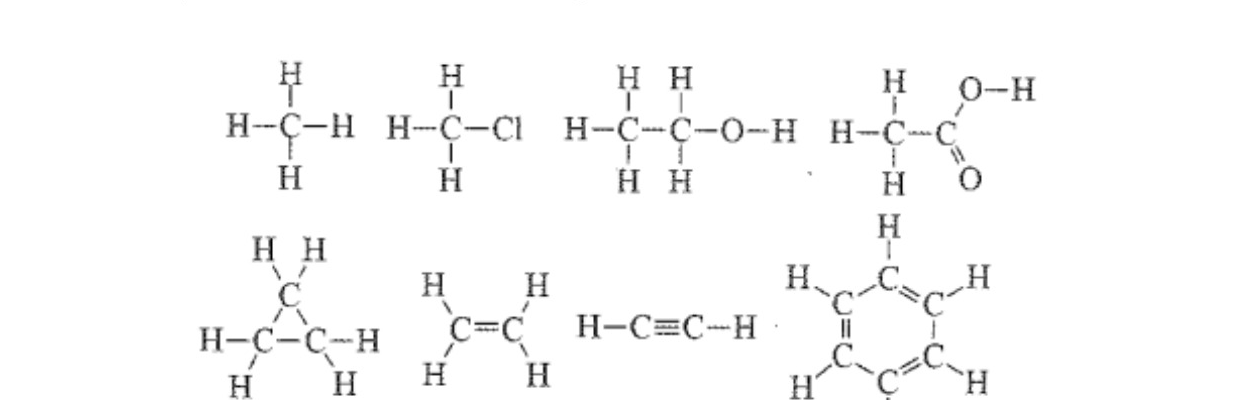
\includegraphics[width=13cm]{images_crop_hoa11_de08/cau9_p1_cau_truc_8chat.png}
\end{center}
Nhận định nào sau đây \textbf{không} đúng?
\choice
{số hydrocarbon bằng 5}
{số dẫn xuất hydrocarbon bằng 3}
{số hydrocarbon no bằng 2}
{\True số hydrocarbon không no bằng 3}

\end{ex}

\begin{ex}
\textbf{[KNTT - SBT]} Nhận định nào sau đây \textbf{không} đúng?
\choice
{$\ce{CH4, CH2=CH2}$ và $\ce{CH#CH}$ là những hydrocarbon}
{$\ce{CH3OH}$ và $\ce{HOCH2-CH2OH}$ là những alcohol}
{$\ce{CH3COOH}$ và $\ce{CH2(COOH)2}$ là những carboxylic acid}
{\True $\ce{CH3CH=O}$ và $\ce{CH3COCH3}$ là những aldehyde}

\end{ex}

\begin{ex}
\textbf{[KNTT – SBT]} Trong quá trình chưng cất dầu thô, người ta thu được nhiều phân đoạn dầu mỏ, trong đó có xăng (thành phần chính là hỗn hợp các hydrocarbon có số nguyên tử C từ 4 đến 12, nhiệt độ sôi khoảng từ $40^\circ\text{C}$ đến $200^\circ\text{C}$) và dầu hoả (thành phần chính là hỗn hợp các hydrocarbon có số nguyên tử C từ 12 đến 16, nhiệt độ sôi khoảng từ $200^\circ\text{C}$ đến $250^\circ\text{C}$). Sản phẩm thu được ở $150^\circ\text{C}$ đến $200^\circ\text{C}$ là
\choice
{xăng}
{dầu hoả}
{\True xăng và dầu hoả}
{dầu hoả và xăng}

\end{ex}

\begin{ex}
\textbf{[KNTT – SBT]} Thêm benzene vào ống nghiệm đựng dung dịch nước bromine. Sau một thời gian quan sát thấy màu đỏ nâu của bromine
\choice
{chủ yếu trong lớp nước}
{\True chủ yếu trong lớp benzene}
{phân bố đồng đều ở hai lớp}
{bị mất màu hoàn toàn}

\end{ex}

\begin{ex}
\textbf{(SBT - CĐ)} Sau khi biết công thức thực nghiệm, có thể xác định công thức phân tử của hợp chất hữu cơ dựa trên đặc điểm nào sau đây?
\choice
{\True Phân tử khối của chất}
{Thành phần phần trăm về khối lượng của các nguyên tố có trong phân tử chất}
{Khối lượng các sản phẩm thu được khi đốt cháy hoàn toàn một lượng chất xác định}
{Các hấp thụ đặc trưng trên phổ IR của chất}

\end{ex}

\begin{ex}
\textbf{(SBT - KNTT)} Hình sau đây là phổ khối lượng của phân tử acetic acid:
\begin{center}
	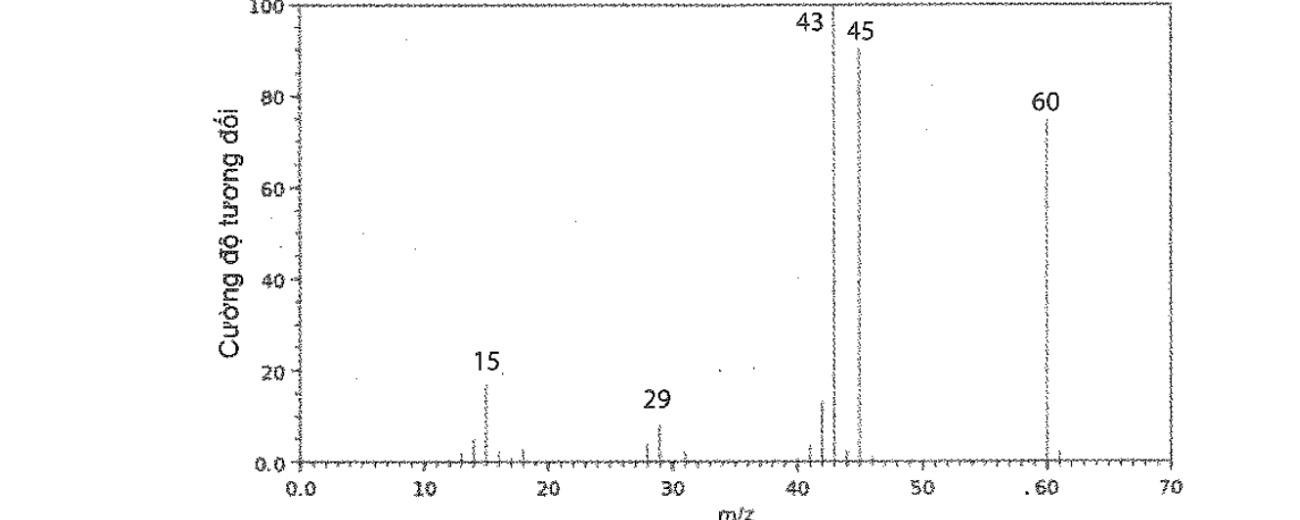
\includegraphics[width=9cm]{images_crop_hoa11_de08/cau14_p1_ms_acetic_acid.png}
\end{center}
Phân tử khối của acetic acid bằng
\choice
{43}
{45}
{\True 60}
{29}

\end{ex}

\begin{ex}
Cho các cặp chất:
\begin{enumerate}[(1)]
	\item $\ce{CH3CH2OH}$ và $\ce{CH3OCH3}$
	\item $\ce{CH3CH2Br}$ và $\ce{BrCH2CH3}$
	\item $\ce{CH2=CH-CH2OH}$ và $\ce{CH3CH2CHO}$
	\item $\ce{(CH3)2NH}$ và $\ce{CH3CH2NH2}$
\end{enumerate}
Có bao nhiêu cặp là đồng phân cấu tạo?
\choice
{1}
{2}
{\True 3}
{4}

\end{ex}

\begin{ex}
Cho chất acetylene ($\ce{C2H2}$) và benzene ($\ce{C6H6}$), hãy chọn nhận xét \textbf{đúng} trong các nhận xét sau đây:
\choice
{Hai chất đó giống nhau về công thức phân tử và khác nhau về công thức đơn giản nhất}
{\True Hai chất đó khác nhau về công thức phân tử và giống nhau về công thức đơn giản nhất}
{Hai chất đó khác nhau về công thức phân tử và khác nhau về công thức đơn giản nhất}
{Hai chất đó có cùng công thức phân tử và cùng công thức đơn giản nhất}

\end{ex}

\begin{ex}
Methadone là một loại thuốc dùng trong cai nghiện ma túy, nó thực chất cũng là một loại chất gây nghiện nhưng ``nhẹ'' hơn các loại ma túy thông thường và dễ kiểm soát hơn. Công thức cấu tạo của methadone như hình dưới:
\begin{center}
	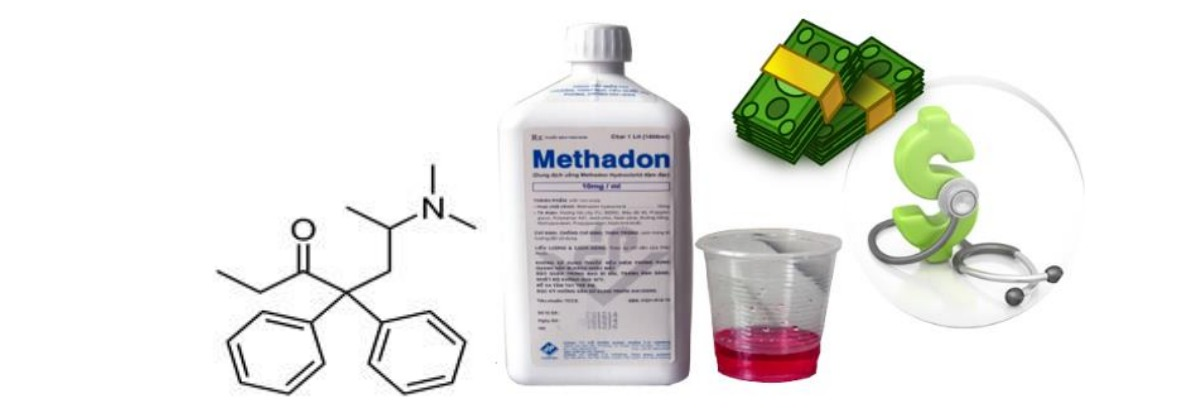
\includegraphics[width=10.5cm]{images_crop_hoa11_de08/cau17_p1_methadone.png}
\end{center}
Công thức phân tử của methadone là
\choice
{$\ce{C17H27NO}$}
{$\ce{C17H22NO}$}
{$\ce{C21H29NO}$}
{\True $\ce{C21H27NO}$}

\end{ex}

\begin{ex}
Cho các phát biểu về đặc điểm chung của các phân tử hợp chất hữu cơ:
\begin{enumerate}[(a)]
	\item Thành phần nguyên tố chủ yếu là C và H.
	\item Có thể chứa nguyên tố khác như Cl, N, P, O.
	\item Liên kết hóa học chủ yếu là liên kết cộng hoá trị.
	\item Liên kết hoá học chủ yếu là liên kết ion.
	\item Dễ bay hơi, khó cháy.
	\item Phản ứng hoá học xảy ra nhanh.
\end{enumerate}
Các phát biểu đúng là
\choice
{4}
{\True 3}
{2}
{1}

\end{ex}

\Closesolutionfile{ans}
\newpage

\noindent\textbf{\large PHẦN II. Câu trắc nghiệm đúng sai.}
\textit{Thí sinh trả lời từ câu 1 đến câu 4. Trong mỗi ý a), b), c), d) ở mỗi câu, thí sinh chọn đúng hoặc sai.}
\vspace{0.2cm}

\begin{ex}
Đặc điểm chung của các phân tử hợp chất hữu cơ:
\choiceTF
{\True a) Thành phần nguyên tố chủ yếu là C và H}
{\True b) Liên kết hóa học chủ yếu là liên kết cộng hoá trị}
{c) Liên kết hoá học chủ yếu là liên kết ion}
{d) Dễ bay hơi, khó cháy}

\end{ex}

\begin{ex}
Một mẫu hoa hoè được xác định có hàm lượng rutin là 26\%. Người ta đun sôi hoa hoè với nước ($100^\circ\text{C}$) để chiết lấy rutin. Biết độ tan của rutin là 5,2 gam trong 1 lít nước ở $100^\circ\text{C}$ và là 0,125 gam trong 1 lít nước ở $25^\circ\text{C}$.
\choiceTF
{a) Trong 100 gam hoa hòe có 30 gam rutin}
{\True b) Cần dùng tối thiểu 5 lít nước để chiết được lượng rutin có trong 100 gam hoa hoè}
{c) Giả thiết rằng toàn bộ lượng rutin trong hoa hoè đã tan vào nước khi chiết. Làm nguội dung dịch chiết 100 gam hoa hoè ở trên từ $100^\circ\text{C}$ xuống $25^\circ\text{C}$ thì thu được 28,0 gam rutin kết tinh}
{\True d) Khi tăng lượng nước, lượng rutin hoà tan trong dung dịch ở $25^\circ\text{C}$ tăng lên nên lượng rutin kết tinh bị giảm đi}

\end{ex}

\begin{ex}
Khi nghiên cứu thành phần hoá học của tinh dầu quế, người ta thu được nhiều hợp chất hữu cơ trong đó có cinnamaldehyde và o–methoxycinnamaldehyde với công thức cấu tạo:
\begin{center}
	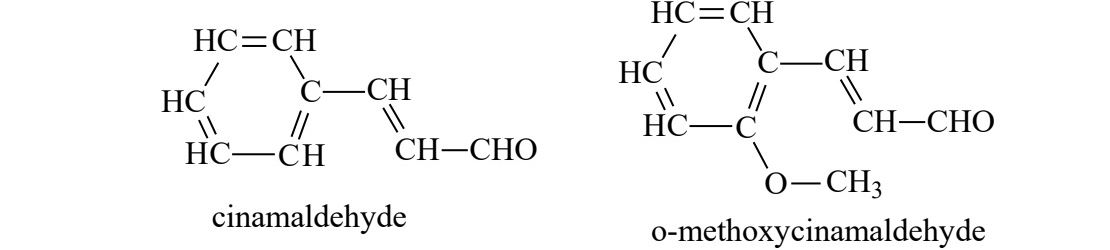
\includegraphics[width=11cm]{images_crop_hoa11_de08/cau3_p2_cinnamaldehyde.png}
\end{center}
Hãy chọn phát biểu Đúng hoặc Sai:
\choiceTF
{\True a) Công thức phân tử cinnamaldehyde: $\ce{C9H8O}$}
{\True b) Công thức đơn giản nhất cinnamaldehyde: $\ce{C9H8O}$}
{c) Công thức phân tử o–methoxycinnamaldehyde: $\ce{C5H5O}$}
{d) Công thức đơn giản nhất: $\ce{C10H10O2}$}

\end{ex}

\begin{ex}
Vanilin là hợp chất thiên nhiên, được sử dụng rộng rãi với chức năng phụ gia bổ sung hương thơm trong các loại đồ ăn, đồ uống, bánh kẹo, nước hoa,... Vanilin có cấu tạo như sau:
\begin{center}
	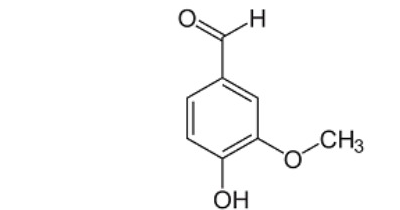
\includegraphics[width=4.5cm]{images_crop_hoa11_de08/cau4_p2_vanilin.png}
\end{center}
\choiceTF
{\True a) Phân tử vanilin có nhóm chức aldehyde}
{b) Phân tử vanilin có chứa nhóm chức alcohol}
{\True c) Vanilin có công thức phân tử $\ce{C8H8O3}$}
{\True d) Vanilin thuộc loại hợp chất hữu cơ tạp chức}

\end{ex}

\vspace{0.2cm}
\noindent\textbf{\large PHẦN III. Câu trắc nghiệm yêu cầu trả lời ngắn.}
\textit{Thí sinh trả lời từ câu 1 đến câu 6.}
\vspace{0.2cm}

\begin{ex}
Có bao nhiêu hydrocarbon trong số các chất dưới đây:
\[ \ce{CH4, NH3, C2H2, CCl4, C2H4, C6H6} \]

\vfill\noindent\textbf{Đáp số:} \dotfill

\end{ex}

\begin{ex}
Cây neem (cây thường xanh Ấn Độ) hay còn gọi là cây nim, sầu đâu (tên khoa học \textit{Azadirachta indica}) được người Ấn Độ dùng hơn 4000 năm nay để làm đẹp và chữa bệnh. Các chiết xuất từ lá neem có thể ức chế sự sao chép của virus Dengue, kháng virus nên có tác dụng điều trị bệnh sốt xuất huyết hiệu quả. Người ta hái một ít lá neem tươi, rửa sạch, cho vào nồi đun kĩ, lọc lấy nước để sử dụng. Hãy cho biết cách làm trên thuộc loại phương pháp tách và tinh chế nào (số thứ tự nào) trong các phương pháp sau:
\begin{center}
	1) Chưng cất; \quad 2) Chiết; \quad 3) Kết tinh; \quad 4) Sắc kí
\end{center}

\vfill\noindent\textbf{Đáp số:} \dotfill

\end{ex}

\begin{ex}
Phổ khối lượng của hợp chất hữu cơ X thu được như hình vẽ:
\begin{center}
	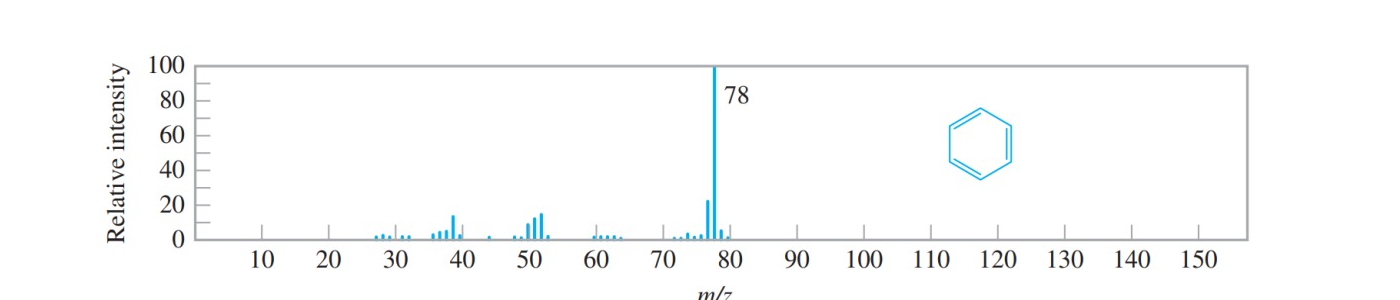
\includegraphics[width=10.5cm]{images_crop_hoa11_de08/cau3_p3_ms_benzene.png}
\end{center}
Phân tử khối của hợp chất hữu cơ X là?

\vfill\noindent\textbf{Đáp số:} \dotfill

\end{ex}

\begin{ex}
Cho công thức sau:
\begin{center}
	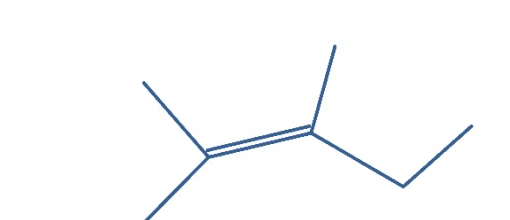
\includegraphics[width=5.5cm]{images_crop_hoa11_de08/cau4_p3_khung_alkene.png}
\end{center}
Hợp chất này có tổng số nguyên tử Carbon và Hydrogen là bao nhiêu?

\vfill\noindent\textbf{Đáp số:} \dotfill

\end{ex}

\begin{ex}
Cho quy trình thực hiện thí nghiệm tinh chế benzoic acid:\\
Cân chính xác 1 gam benzoic acid thô cho vào bình định mức 250 mL. Cho từ từ nước sôi vào bình định mức và lắc đều cho đến khi benzoic acid tan hết. Tiến hành lọc nóng, để yên cho dung dịch nguội từ từ benzoic acid sẽ kết tinh. Lọc bằng máy hút chân không, thu được $m$ gam benzoic acid. Hiệu suất của quá trình kết tinh trên là 40\%. Giá trị của $m$ là bao nhiêu? (kết quả làm tròn đến hàng phần chục).

\vfill\noindent\textbf{Đáp số:} \dotfill

\end{ex}

\begin{ex}
Camphor (có trong cây long não) là một chất rắn kết tinh màu trắng hay trong suốt giống như sáp với mùi thơm đặc trưng, thường dùng trong y học. Phần trăm khối lượng các nguyên tố trong camphor lần lượt là 78,94\% carbon, 10,53\% hydrogen và 10,53\% oxygen. Từ phổ khối lượng của camphor xác định được giá trị $m/z$ của peak $[\ce{M+}]$ bằng 152. Xác định số lượng nguyên tử của camphor.
\begin{center}
	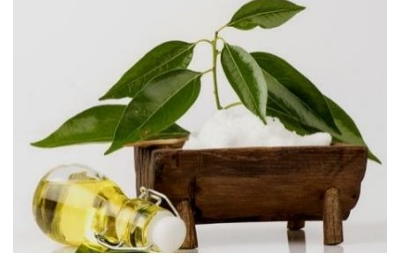
\includegraphics[width=4.5cm]{images_crop_hoa11_de08/cau6_p3_cay_long_nao.png}
	\qquad
	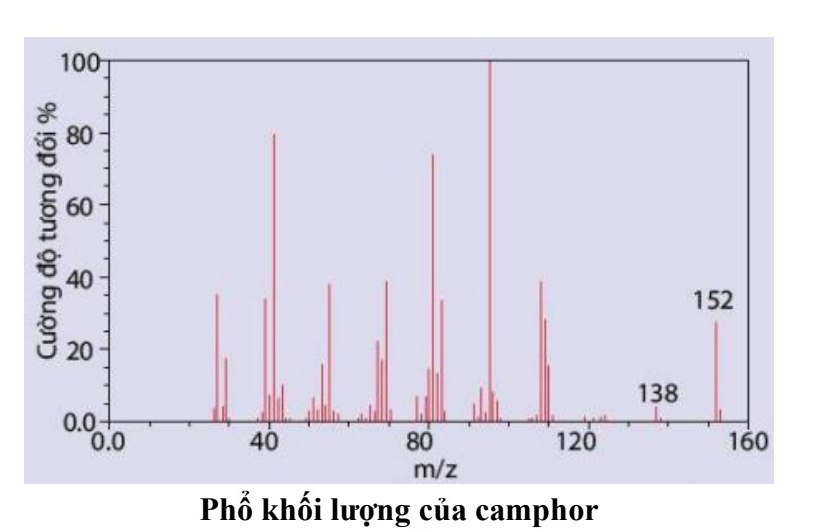
\includegraphics[width=9cm]{images_crop_hoa11_de08/cau6_p3_ms_camphor.png}
\end{center}

\vfill\noindent\textbf{Đáp số:} \dotfill

\end{ex}

\vspace{0.2cm}
\noindent\textbf{\large PHẦN IV. Tự luận.}
\textit{Thí sinh trình bày lời giải chi tiết cho các câu hỏi sau.}
\vspace{0.2cm}

\begin{ex}
\textbf{[CĐ-SGK]} Hãy xác định công thức đơn giản nhất của các hợp chất có công thức dưới đây:
\begin{enumerate}[a)]
	\item $\ce{C4H10}$ (butane)
	\item $\ce{HOCH2CH2OH}$ (ethane-1,2-diol)
	\item $\ce{C6H6}$ (benzene)
	\item $\ce{CHCl2COOH}$ (dichloroethanoic acid)
\end{enumerate}

\noindent\dotfill\\
\noindent\dotfill\\
\noindent\dotfill\\
\noindent\dotfill\\
\noindent\dotfill\\
\noindent\dotfill

\end{ex}

\begin{ex}
\textbf{[SBT - CTST]} Acetic acid được sử dụng rộng rãi trên thế giới trong nhiều ngành công nghiệp khác nhau như tạo ra polymer ứng dụng trong sơn, chất kết dính, là dung môi hoà tan các chất hoá học, sản xuất và bảo quản thực phẩm đặc biệt dùng để sản xuất giấm.
\begin{enumerate}[a)]
	\item Lập công thức phân tử của acetic acid, biết kết quả phân tích nguyên tố của acetic acid có 40\% C; 53,33\% O về khối lượng; còn lại là H. Phân tử khối của acetic acid được xác định trên phổ khối lượng tương ứng với peak có giá trị $m/z$ lớn nhất.
	\begin{center}
		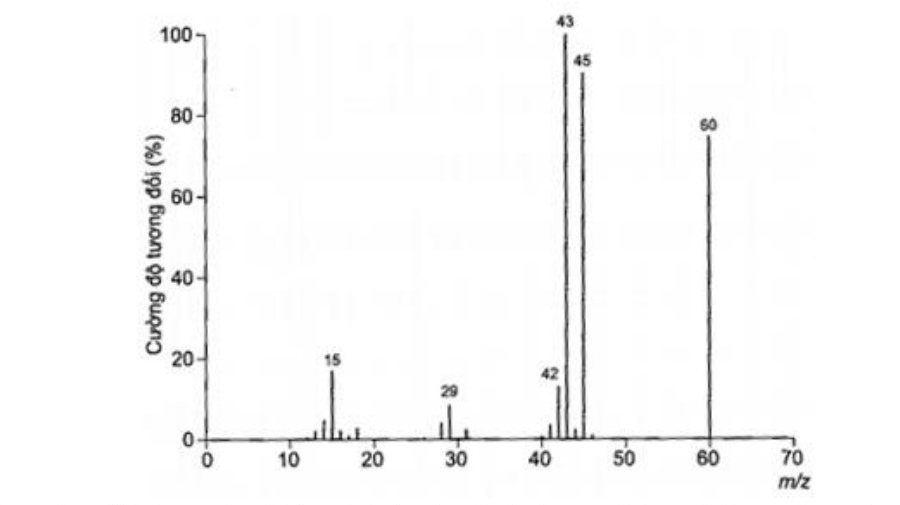
\includegraphics[width=9cm]{images_crop_hoa11_de08/cau2_p4_ms_acetic_acid.png}
	\end{center}
	\item Dựa vào phổ IR bên, hãy cho biết có thể xác định được nhóm chức carboxyl có trong acetic acid từ peak nào.
	\begin{center}
		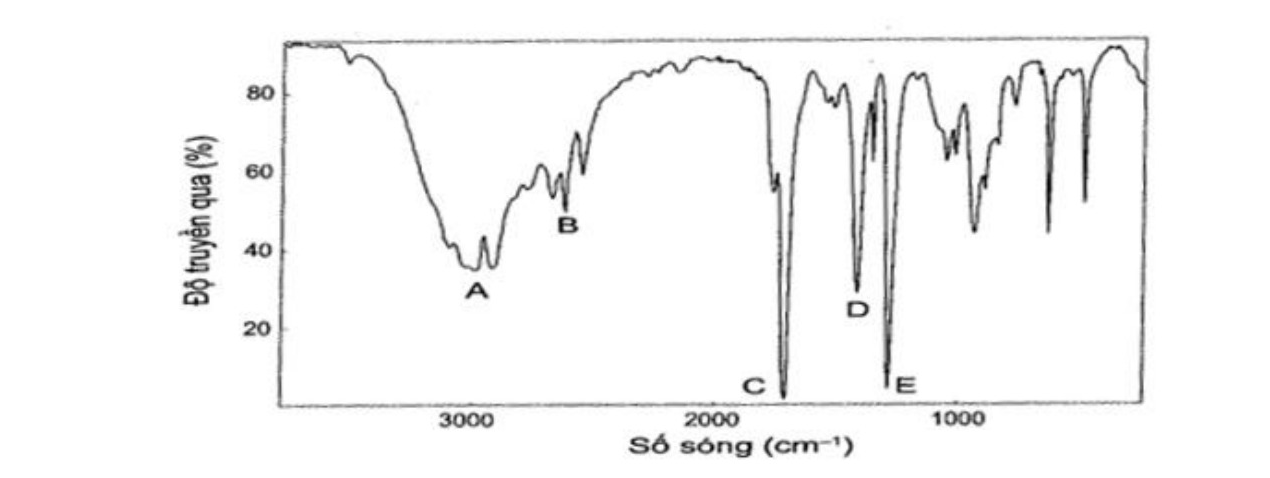
\includegraphics[width=11cm]{images_crop_hoa11_de08/cau2_p4_ir_acetic_acid.png}
	\end{center}
\end{enumerate}

\noindent\dotfill\\
\noindent\dotfill\\
\noindent\dotfill\\
\noindent\dotfill\\
\noindent\dotfill\\
\noindent\dotfill\\
\noindent\dotfill\\
\noindent\dotfill

\end{ex}

\begin{center}
\textbf{--------- HẾT ---------}
\end{center}

\end{document}
